% Generated from tex/chapters/ch04/07_実務上の考慮.tex for the SWEBOK structure tree
\subsubsection{構築言語}

構築言語とは、人間がコンピュータに実行可能な解決策を指定するための言語である。狭い意味のプログラミング言語だけでなく、設定言語、ツールキット言語、スクリプト言語、ドメイン固有言語も含む。

\par\smallskip\noindent\refstepcounter{table}\label{tab:ch04-03}\textbf{表 \thetable: 第04章 ソフトウェア構築 表03}\par\smallskip
\begin{longtable}{L{0.24\linewidth}L{0.66\linewidth}}
\toprule
\textbf{構築言語の種類} & \textbf{説明} \\
\midrule
設定言語 & 限られた選択肢から設定を選び、ソフトウェアの振る舞いや導入形態を変える言語である。設定ファイルなどが該当する。 \\
ツールキット言語 & 特定の部品群やツールキットを組み合わせてアプリケーションを作るための言語である。 \\
スクリプト言語 & 自動化、処理の連結、簡易アプリケーションの構築によく使われる言語である。 \\
プログラミング言語 & 汎用的で柔軟な構築言語である。C/C++、Java、Python、C\# などが例である。 \\
ドメイン固有言語 & 特定の業務領域や技術領域の概念を直接表す言語である。汎用言語よりも領域内の問題を簡潔に表せることがある。 \\
\bottomrule
\end{longtable}

構築言語の表記法には、テキストを中心にする言語的表記、数学的に厳密な形式的表記、図形やアイコンを中心にする視覚的表記がある。言語選択は、性能、信頼性、移植性、セキュリティ、開発者の学習コストに影響する。

\begin{figure}[htbp]
\centering
\IfFileExists{assets/fig-ch04-06.png}{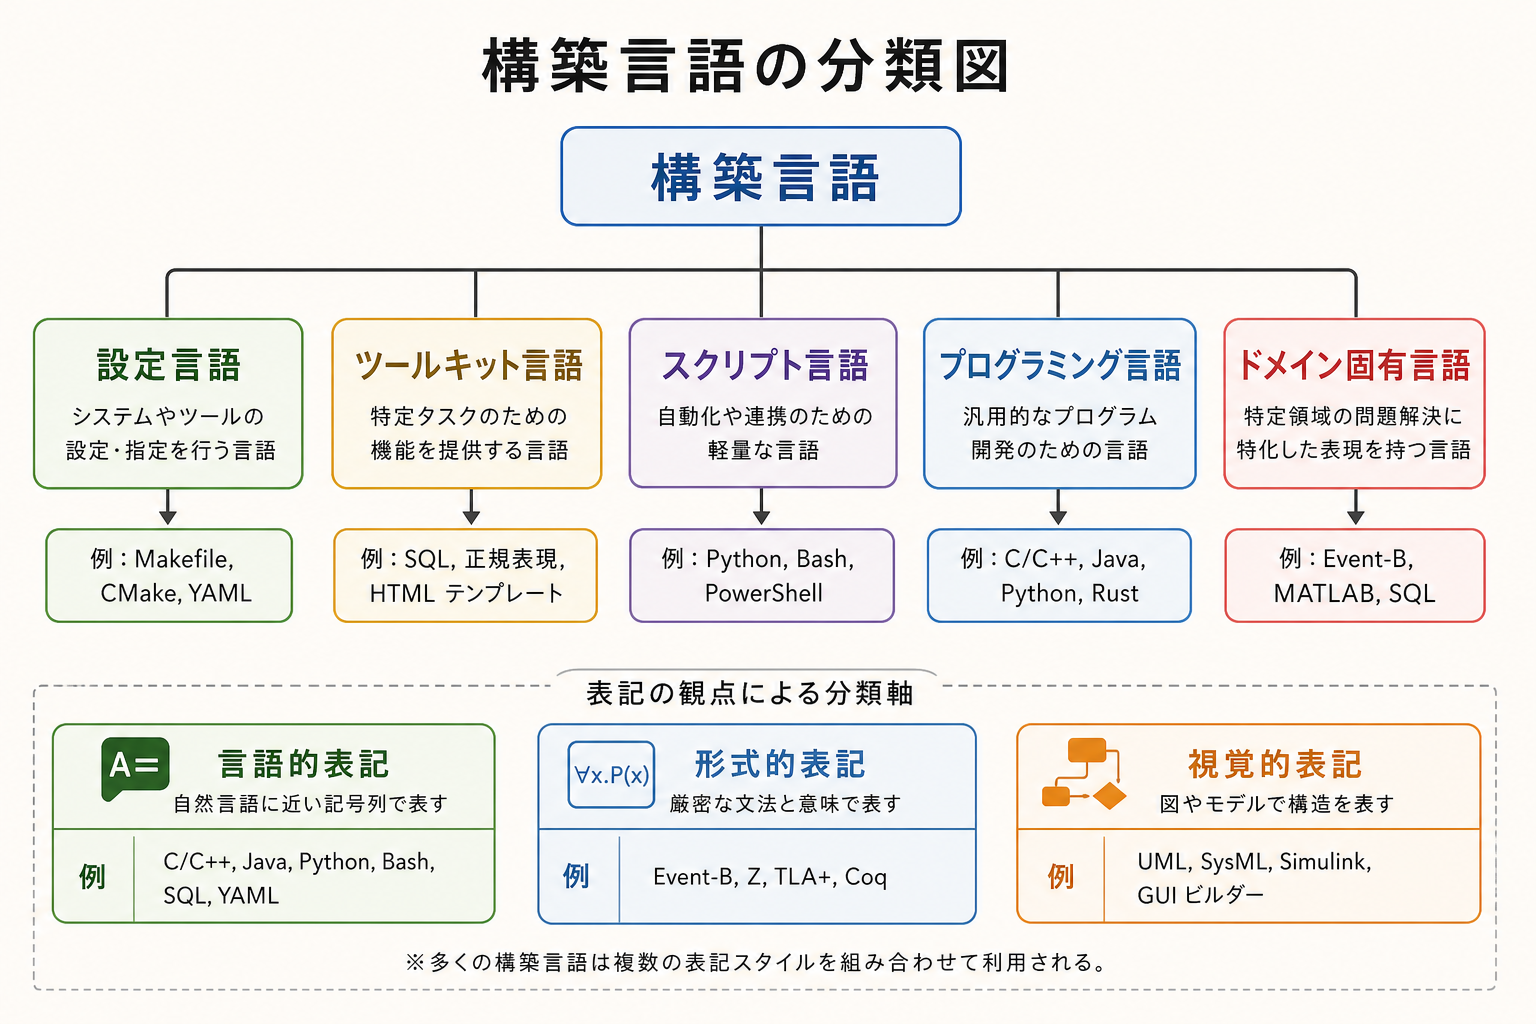
\includegraphics[width=0.96\linewidth]{assets/fig-ch04-06.png}}{\fbox{\parbox[c][48mm][c]{0.9\linewidth}{\centering 画像生成待ち\\構築言語の分類図}}}
\caption{構築言語の分類図}
\label{fig:ch04-06}
\end{figure}
